

%!TEX root = ./main.tex
\chapter{Approach
\label{chapter:approach}}

\section{Methodology
\label{section:methodology}}

To achieve the goal of enhancing the traffic preselection of FACT with
knowledge about the past stability and popularity characteristics, the following
three steps are planned for extending FACT as illustrated in figure
\ref{fig:FACT}.
\begin{figure}
	[ht] \centering
	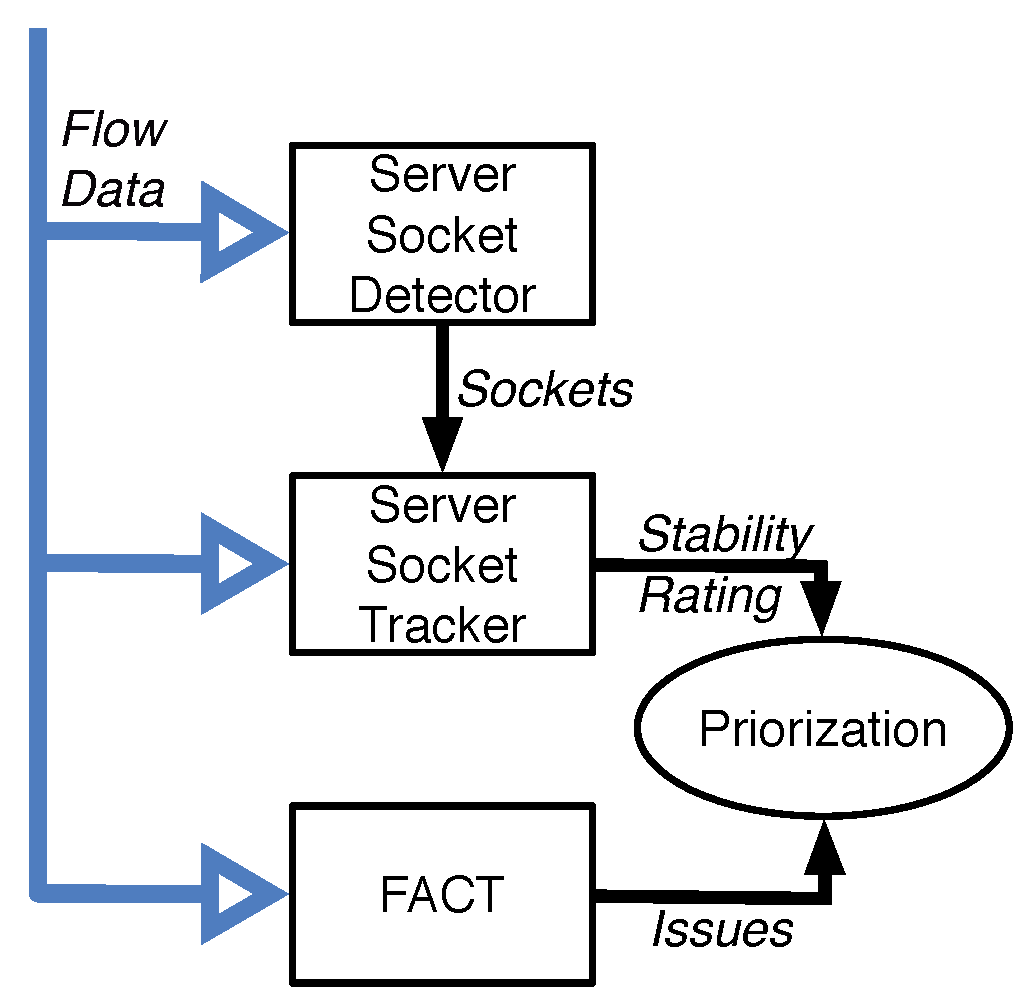
\includegraphics[width=8.5cm]{images/Approach_blockdiagram.eps}
	\caption{Interactions of new components with FACT} 
	\label{fig:FACT} 
\end{figure}

In a first step, a server socket detector is implemented. The challenge of the
server socket detection lies in the fact that the netflow data does not provide
enough precise timing information to determine which flow is originated from the
client and thus determine the server's socket. Therefore, the server socket
detection is achieved by the assumption that server sockets act as concentrators
in the sense that several clients have connections to the identical server
socket and bases on the work shown in
\cite{Schatzmann:Dissection,Schatzmann:Mining,Schatzmann:Tracing} and is
discussed in more detail in section \ref{section:socket_detection}.

Secondly, the previously detected server sockets are continually monitored and
especially the successful and unsuccessful connection attempts are recorded by
the server socket tracker.
Furthermore, these information are used to update the statistical information of
visibility, popularity and stability. Section \ref{section:socket_tracking}
covers this step in detail.

In a third step, the number of server sockets have to be reduced by selecting a 
set of suitable server sockets such that FACT is able to use these sockets for 
outage tracking. In particular, the server socket sets coverage of the Internet 
address space has to be assessed, because it makes for example no sense to 
select only the most popular sockets if they are all located in the same /24 
network.

Finally, FACT has to be adopted to optimally use the preselected and rated
server sockets for prioritizing relevant connectivity issues by reducing outage
alerts based on single host outages of unstable services.

%%%%%%%%%%%%%%%%%%%%%%%%%%%%%%%%%%%%%%%%%%%%%%%%%%%%%%%%%%%%%%%%%%%%%%%%%%%%%%%%
\section{Data
\label{section:data}}

This thesis relies on data collected at \citet{switch}, the Swiss National 
Research and Education Network (NREN). Mainly government institutions, 
universities, research labs are connected to the internet by \citet{switch}\citep{Schatzmann:Mining}.

The \citet{switch} network is with approximately 250'000 network users in 2010 comparable with a mid sized ISP. Currently, there are around 2.4 million IPv4 addresses, a /32 IPv6 and a /40 IPv6 network announced via BGP\citep{Schatzmann:Tracing}.

\begin{figure}[h] 
	\centering
	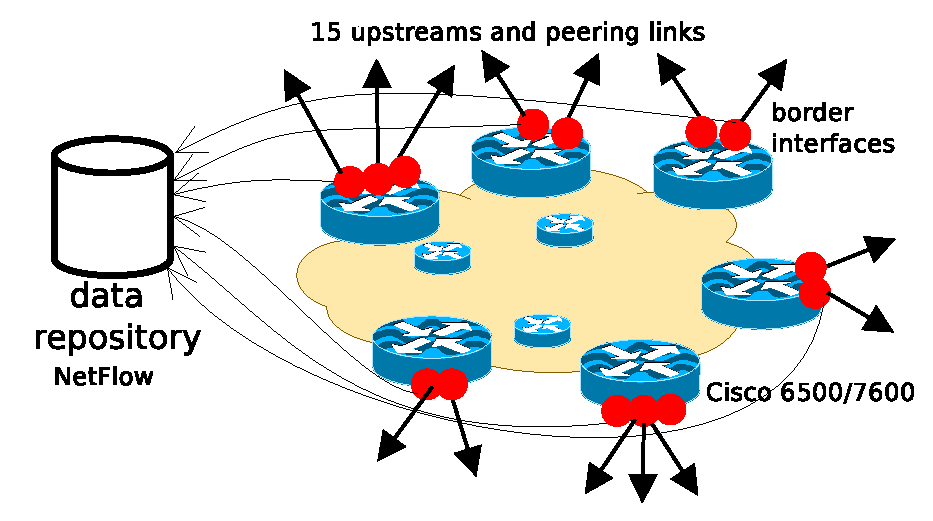
\includegraphics[width=12cm]{images/network_overview.eps}
	\caption{Overview of the SWITCH network \citep{SchatzmanThesis2012}} 
	\label{fig:switch_nework}
\end{figure}

\citet{switch} is capturing flow level data at all external interfaces of their border routers by 2003 in form of unsampled NetFlow data -- from 2003-2008 in version 5 and in version 9 after 2008\citep{Schatzmann:Tracing}.
High traffic peak rates of more than 80'000 flows per second, 3 million packets per second and more than 20Gbit/s require hardware-based flow collection cards. TCP flags are not available in the flow level information because of some limitations of these hardware components. The generated flow data is collected and stored at a central data repository.

Figure \ref{fig:switch_nework}

% briefly describe the Switch network and its topology..
% traffic volume and netflow data unsampled!
% see tech report 338 for numbers and layout?! evtl actual numbers (2012)
%%%%%%%%%%%%%%%%%%%%%%%%%%%%%%%%%%%%%%%%%%%%%%%%%%%%%%%%%%%%%%%%%%%%%%%%%%%%%%%%